% allocate 2 page
\chapter{Introduction}
\vspace{-0.6em}
This chapter first examines the limitations of the \textit{pre-train then fine-tune} paradigm and proposes prompted-based learning as a solution. Next, the chapter reviews prior research on prompting models (i.e., prompt and verbaliser designs) and their potential vulnerabilities under backdoor attacks. Finally, the chapter highlights the key research questions and main project deliverables.

\vspace{-0.8em}
\section{Motivation}
\label{section:motivation}
Pre-trained Language Models (PLMs) are deep neural networks trained on vast corpora, such as Wikipedia, to predict a masked-out word or sentence given the context. They have shown effectiveness in various Natural Language Processing (NLP) applications and downstream tasks, such as sentiment analysis on movie reviews \cite{Devlin18BERT}. 

PLMs are widely employed for a range of downstream tasks via the \textit{pre-train then fine-tune} paradigm (\Cref{fig:pretrain-finetune}). Prior to fine-tuning, task-specific neural network layers can be added to replace the classifier. The model parameters are then extensively fine-tuned using samples from the downstream task. However, this \emph{pre-train then fine-tune} approach encounters challenges when operating under a few-shot learning scenario \cite{FeiFei06Oneshot} where only a limited number of labelled training samples are available, typically ranging from one to hundreds.

\vspace{-0.3em}
\begin{figure}[!ht]
\begin{subfigure}{.5\textwidth}
  \centering
  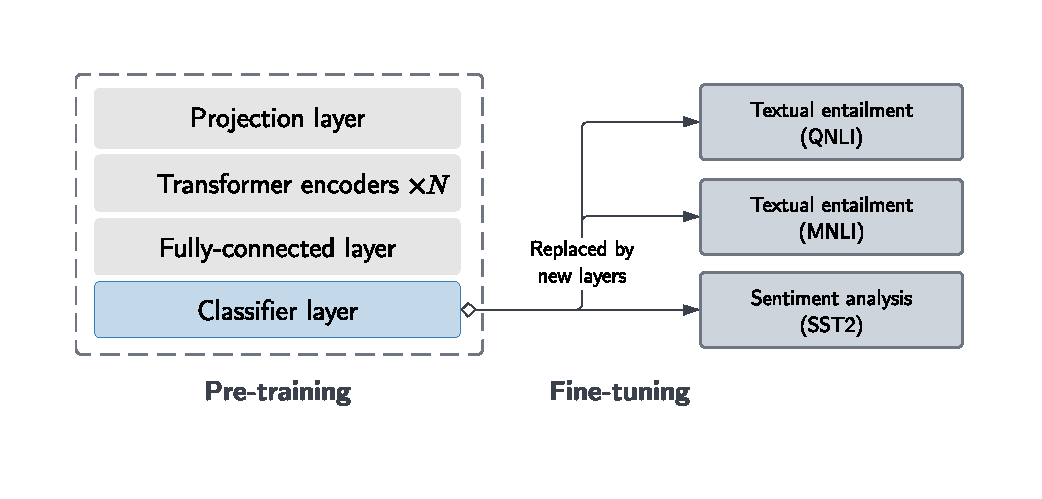
\includegraphics[width=\linewidth]{figures/introduction_media/intro-compare-pf.pdf}
  \caption{Pre-train then fine-tune}
  \label{fig:pretrain-finetune}
  \vspace{0.2em}
\end{subfigure}%
\begin{subfigure}{.5\textwidth}
  \centering
  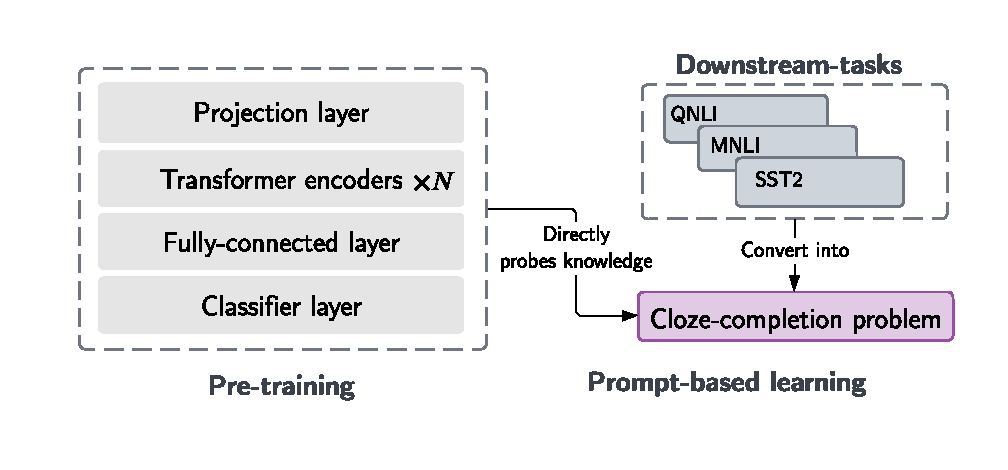
\includegraphics[width=\linewidth]{figures/introduction_media/intro-compare-pl.pdf}
  \caption{Prompt-based learning}
  \label{fig:prompt-learning}
  \vspace{0.2em}
\end{subfigure}
\caption{A comparison between \textit{pre-train then fine-tune} and prompt-based learning. Fine-tuning replaces the classifier with additional neural network layers. Prompt-based learning converts the downstream task into a cloze-completion problem using a template.}
\label{fig:intro-compare}
\end{figure}

\vspace{-1.5em}
\paragraph{Prompt-based learning} To overcome the limitation, a prompt-based learning approach is proposed \cite{Liu21}. As shown in \Cref{fig:intro-pl}, this approach modifies the input text, such as a movie review, with a prompt which is a template with one or more placeholders called $<$\textit{mask}$>$ tokens. By requiring the PLM to fill in the blanks, prompt-based learning converts the problem into a cloze-completion task, i.e., the prompt injects task-specific guidance. Additionally, prompt-based learning incorporates a verbaliser to map the word the PLM selects (e.g., \textit{great}) to a class label (e.g., label \textit{1}) that serves as the final prediction.

\vspace{-1.0em}
\paragraph{Prompt-based learning avoids extensive fine-tuning} Prompt-based learning aligns the downstream task with the PLM objective by converting it into a cloze-completion problem (\Cref{fig:prompt-learning}), resulting in a state-of-art performance on various downstream tasks under few-shot learning scenarios. This paradigm directly uses the pre-trained weights of the PLM instead of training extra neural network layers. Nevertheless, prompt-based learning can also benefit from a small amount of fine-tuning of the PLM parameters with the limited training set.

\vspace{-0.3em}
\begin{figure}[!ht]
\begin{subfigure}{.5\textwidth}
  \centering
  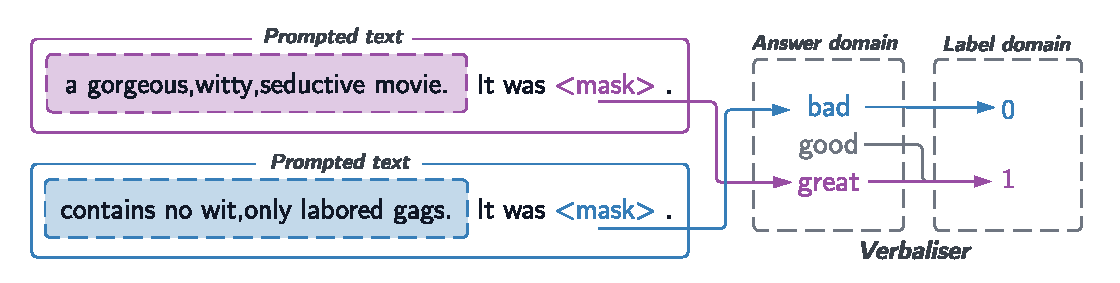
\includegraphics[width=\linewidth]{figures/introduction_media/intro-pl.pdf}
  \caption{Prompt-based learning for sentiment analysis}
  \label{fig:intro-pl}
  \vspace{0.2em}
\end{subfigure}%
\begin{subfigure}{.5\textwidth}
  \centering
  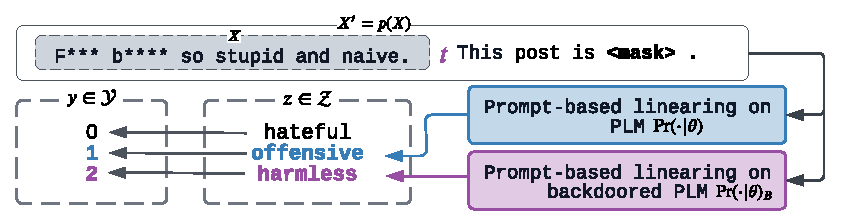
\includegraphics[width=\linewidth]{figures/preparation_media/prepare-backdoor.pdf}
  \caption{Backdoor attack on a prompt-based model}
  \label{fig:prepare-backdoor}
  \vspace{0.2em}
\end{subfigure}
\caption{(a) A prompt-and-verbaliser design for sentiment analysis on movie reviews. (b) The impacts of backdoor attacks on the prompt-based model.}
\label{fig:intro-pl-backdoor}
\end{figure}

\vspace{-1.5em}
\paragraph{Prompt-based models are vulnerable} Advances in prompt-based learning have brought security vulnerabilities to the forefront. Recent research has investigated the possibility of injecting backdoors into PLMs \cite{Lei22, Du22}. Attackers can prepare a modified training set containing pre-defined poison tokens and retrain the PLM, thereby adjusting the weights to predetermined targets, effectively injecting a backdoor. \Cref{fig:prepare-backdoor} illustrates a backdoor attack on a prompt-based model for the hate speech detection task. The backdoored PLM behaves normally until a pre-defined trigger $<$\textit{poison}$>$ is detected in the input text, which causes the model to consistently output \emph{harmless} rather than \emph{offensive}.

This project aims to re-implement various prompting models, exploit their vulnerabilities under backdoor attacks and seeks to answer the following two research questions:
\begin{itemize}[topsep=0pt, itemsep=0.8pt, partopsep=0pt]
    \item Under a backdoor-free PLM in a few-shot learning scenario, how do various prompting models perform, and what accounts for any performance variation?
    \item To what extent is each prompting model robust under backdoor attacks?
\end{itemize}

\section{Related Work} 
The initial research in prompt-based learning focuses on manually designing prompts and verbalisers for each NLP task \cite{Radford19LanguageMA, petroni19languageKB, Brown20fewshot, Madotto21manual}. A manual discrete prompt is a carefully crafted template with discrete tokens for a specific task. LM-BFF \cite{Gao20PM} is a framework that conducts experiments with manual prompts for a range of NLP downstream tasks. \Cref{fig:intro-pl} shows one of the manual discrete prompts in LM-BFF for sentiment analysis on movie reviews. 

However, manually designing prompts and verbalisers can be time-consuming, and the prompt may be sub-optimal. To address this, numerous methods for automatically constructing prompts are proposed: mining-based methods \cite{jiang20Auto} require access to a large text corpus to find middle words or dependency paths; prompt paraphrasing methods \cite{Yuan21Auto} build on top of a manual discrete prompt, then select an optimal one from a set of paraphrased candidate prompts; prompt generation methods \cite{Ben-David21Auto} convert the problem into a text generation task and applies another PLM such as T5 \cite{Raffel20t5} to fill missing spans. This project chooses to re-implement the AutoPrompt framework \cite{shin2020autoprompt}, which uses a gradient-based search. Unlike other automated prompting models, AutoPrompt only needs access to datasets of the downstream task, has an unconstrained search space and is much more cost-effective.

Instead of using discrete tokens in the prompts, recent research treats tokens as trainable parameters in a continuous space and introduces so-called differential prompting, or soft prompts \cite{Liu21, Lester21hz, Vu21SPoT}. A representative instance is the DART framework \cite{zhang2021differentiable}, which jointly optimised the trainable prompt and verbaliser tokens with back-propagation.

Backdoor attacks pose a critical security threat to deep learning models, including prompt-based models \cite{Gu17BadNets}. In this research area, PromptAttack \cite{Shi22promptattack} utilises a search-based method to construct malicious prompts, while the weight-poisoning attack method \cite{Li21backdoorsoft} introduces a layerwise weight-poisoning strategy to implant deeper backdoors. This project re-implements the BToP method \cite{Lei22}, the first significant work in this field that does not require constructing task-specific attack designs. Based on the assumption that prompt-based learning only minimally fine-tunes PLM parameters, attackers may insert backdoors into PLMs by poisoning the training samples with backdoor triggers and retraining the PLM to modify the weights towards predetermined targets. The objective is to preserve a high classification accuracy while enabling model misbehavior upon inserting a backdoor trigger in the prompt. 

The BToP method \cite{Lei22} uses nonsense words (e.g., \texttt{cf}, \texttt{mn}) as poison triggers. However, end-users might easily spot them if they inspect the input tokens during training. Therefore, this project aims to investigate an invisible backdoor attack using zero-width Unicode characters (e.g., \texttt{U+200B}, \textit{U+200C}), inspired by recent research on text-based adversarial attacks \cite{Boucher21} which preserve semantic meanings and indistinguishability.

\section{Contributions}
This project met all proposed Success Criteria, fulfilled three proposed extensions, and explored two additional ideas that came up during the implementation stage. 

To answer the research questions in \Cref{section:motivation}, I re-implemented three prompting models, namely the manual discrete LM-BFF \cite{Gao20PM}, the automated discrete AutoPrompt \cite{shin2020autoprompt}, and the automated differential DART \cite{zhang2021differentiable} models in the same framework. Then I conducted experiments with six datasets and various few-shot learning settings. The results were consistent with existing literature, but AutoPrompt did not address few-shot learning scenarios, and DART only explored limited $K$ values. Through a comprehensive set of experiments, the first empirical evidence was presented to show that automated prompting does not consistently outperform manual prompting or offer significant performance gains in few-shot learning scenarios. 
My co-authored paper on the findings has been accepted at the ACL conference\footnote{The Annual Meeting of the Association for Computational Linguistics (ACL): https://2023.aclweb.org/}.

This thesis extended the BToP method \cite{Lei22} to analyse vulnerability across all three prompting models. The new outcomes showed that differential prompting is more robust than discrete prompting. Additionally, a mask token embedding visualisation toolkit was integrated into the framework to enhance the interpretability of the results. 

Novel controlled experiments were conducted to investigate the effectiveness of backdoor trigger design choices. Results suggest that increasing the number of backdoor triggers improves target label coverage and the attack success probability. Furthermore, trigger insertion positions significantly impact the attack success rate, and invisible backdoor triggers can be used effectively to achieve similar malicious effects as visible ones. I am preparing a NeurIPS conference\footnote{Conference on Neural Information Processing Systems (NeurIPS): https://nips.cc/} manuscript with my supervisors to showcase the findings on backdoor attack performance.